\chapter{The Signature Selection Problem}

Despite the clever search strategies employed by theory exploration tools, they
all rely on enumerating combinations of definitions in some way, which can cause
infeasible running times on larger inputs (in our experience, a few dozen
definitions). To avoid this, users of these systems must carefully select only
small subsets of their definitions to explore at a time.

We dub such selection the \emph{signature selection problem} for theory
exploration, and we analyse its effect on the running time of theory exploration
tools on the TIP particular problem set, and on the quality of the statements
they are able to generate. An automated solution to this signature selection problem would
accept a large number of definitions and efficiently select sub-sets which are
both small enough to reasonably explore, whilst still enabling interesting
properties to be discovered.

In this chapter we will:

\begin{enumerate}
  \item Define the \emph{signature selection problem} for theory exploration.
  \item Analyse the performance of theory exploration on the Theory Exploration
    Benchmark.
  \item Analyse the effect of signature selection on the quantity of desirable properties
    attainable by theory exploration on this problem set.
  \item Demonstrate how the signature selection problem is distinct from the well-know
    \emph{clustering problem} in machine learning, and how clustering algorithms
    cannot be directly applied to signature selection.
\end{enumerate}

Some bespoke components required for these analyses and comparisons may also be
useful on their own, or re-purposed for other tasks. These include:

\begin{enumerate}
\item A novel feature extraction method for transforming Haskell expressions
  into a form amenable to off-the-shelf machine-learning algorithms, based on
  the existing \emph{recurrent clustering} algorithm from other languages.
\item An executable implementation of this feature extraction
  approach\footnote{https://github.com/warbo/ml4hsfe}.
\item End-to-end automation for exploration arbitrary, user-provided Haskell
  packages\footnote{https://github.com/warbo/haskell-te}.
\item Dynamic evaluation of Haskell code, with access to dynamically installed
  Haskell packages\footnote{http://hackage.haskell.org/package/nix-eval}.
\item Translation of the signature selection problem to the constrain-solving domain, and
  executable oracles for optimal (and pessimal) signature selection, when the desired
  properties are already known\footnote{Part of
    https://github.com/warbo/bucketing-algorithms}.
\end{enumerate}

\iffalse
% TODO: Do we need this?
We describe theory exploration in more detail, as well as the \qspec{} tool we
use in our experiments, in \S~\ref{sec:theoryexploration}. We introduce the
signature selection problem more formally in \S~\ref{sec:sigselect} and measure its
effect on theory exploration systems in \S~\ref{sec:implementation}. In
\S~\ref{sec:clustering} we highlight the difference between signature selection and the
well-known \emph{clustering problem} from machine learning, by demonstrating
that clustering algorithms perform poorly at signature selection.  A variety of related
work is surveyed in \S~\ref{sec:related} and we conclude in
\S~\ref{sec:conclusion} with potential directions for future research.
\fi

\section{Background}
\label{sec:background}

As an example, giving the definitions from Figure~\ref{fig:haskellteexample} to
\qspec{}, along with suitable comparison functions, random data generators and
variables \hs{n :: Nat} and \hs{b :: Bool}, will give rise to an equivalence
class for each type \hs{Nat}, \hs{Bool}, \hs{Nat -> Nat}, \hs{Nat -> Bool} and
\hs{Bool -> Bool}. Testing will find unequal terms in some of these classes
(such as the \hs{Bool} class containing \hs{True}, \hs{False}, \hs{b},
\hs{not b}, \hs{odd n} and \hs{even n}, which are all mutually unequal), split
them up, and repeat until no more splits are found. Equations are then generated
between elements of non-singleton classes, such as $\{\text{\hs{odd n}},
\text{\hs{not (even n)}}, \text{\hs{not (not (odd n))}}, \ldots\}$, and reduced
to a minimal set (for example, discarding \hs{odd n == not (not (odd n))} as an
instance of the more general \hs{b == not (not b)}). The remaining equations
(including \hs{not (not b) == b} and \hs{not (odd n) == even n}, etc.) are
output, either for the user to peruse or for another system to process, like the
\textsc{HipSpec} automated theorem prover.

Note that we must be able to generate values of a type in order to include
variables of that type. Also, only equivalence classes whose element type can be
compared are split and conjectured about in this way; in particular, functions
(like \hs{odd} and \hs{even}) are first-class values, so they will be put in an
equivalence class, but they will not be subject to testing and comparison since
Haskell has no generic notion of function equality~\footnote{In
  fact \qspec{} compares expressions using a total ordering rather than equality;
  this is even more restrictive than requiring a notion of equality, but reduces
  the number of required comparisons}. \qspec{} can hence conjecture that two
functions are pointwise-equal (e.g. \hs{f x == g x}) but it cannot conjecture
that the functions themselves are equal (e.g. \hs{f == g}).

Although complete, this enumeration approach is wasteful: many terms are
unlikely to appear in theorems, which requires careful choice by the user of
what to include in the signature. For example, we know that addition and
multiplication are closely related, and hence obey many algebraic laws. Our
machine learning technique aims to predict these kinds of relations between
functions, so we can create small signatures which can be explored quickly, yet
have the potential to give rise to many equations.

\section{Clustering}
\label{sec:clustering}

Our approach to scaling up \qspec{} takes inspiration from two sources. The
first is relevance filtering, which makes expensive algorithms used in theorem
proving more practical by only considering clauses deemed ``relevant'' to the
problem \cite{meng2009lightweight}.

Relevance is determined by comparing clauses to the target theorem, but theory
exploration does not have such a distinguished term. Instead, we are interested
in relationships between \emph{all} terms in a signature, and hence we need a
different algorithm for considering the relevance of \emph{all terms} to
\emph{all other terms}.

A natural fit for this task is \emph{clustering}, which attempts to group
similar inputs together in an unsupervised way. Based on their success in
discovering relationships and patterns between expressions in Coq and ACL2 (in
the ML4PG and ACL2(ml) tools respectively), we hypothesise that clustering
methods can fulfil the role of relevance filters for theory exploration:
intelligently breaking up large signatures into smaller ones more amenable to
brute force enumeration, such that related expressions are explored together.

Due to its use by ML4PG and ACL2(ml), we use \emph{k-means} clustering,
implemented in the Weka tool \cite{Holmes.Donkin.Witten:1994} by Lloyd's
algorithm \cite{lloyd1982least}, with randomly-selected input elements as the
initial clusters. Rather than relying on the user to provide the number of
clusters $k$, we use the ``rule of thumb'' given in
\cite[pp. 365]{mardia1979multivariate} of clustering $n$ data points into
$k = \lceil \sqrt{\frac{n}{2}} \rceil$ clusters.

\subsection{The Signature Selection Problem}
\label{sec:sigselect}

% TODO{2019-04-19}

\subsection{Recurrent Clustering}
\label{sec:recurrentclustering}

Rather than clustering Core expressions directly, we first perform \emph{feature
  extraction} to transform them into numeric \emph{feature vectors}. We adapt
the methodology of \emph{recurrent clustering} proposed in
\cite{DBLP:journals/corr/HerasK14} \cite{heras2013proof}, which combines feature
extraction and clustering into a single recursive algorithm, such that the
feature vector of an expression depends on the feature vectors of those
expressions it references. We suggest a new recurrent clustering and feature
extraction algorithm for Haskell (shown in Algorithm \ref{alg:recurrent}) and
compare its similarity and differences to those of ML4PG and ACL2(ml).

We describe our algorithm in two stages: the first transforms the nested
structure of expressions into a flat vector representation; the second converts
the discrete symbols of Core syntax into features (real numbers), which we will
denote using the function $\phi$.

\subsubsection{Expressions to Vectors}
\label{sec:expressionstovectors}

Our recurrent clustering algorithm is based on k-means clustering, which
considers the elements of a feature vector to be \emph{orthogonal}. Hence we
must ensure that similar expressions not only give rise to similar numerical
values, but crucially that these values appear \emph{at the same position} in
the feature vectors. Since different patterns of nesting can alter the ``shape''
of expressions, simple traversals (breadth-first, depth-first, post-order, etc.)
may cause features from equivalent sub-expressions to be mis-aligned. For
example, consider the following expressions, which represent pattern-match
clauses with different patterns but the same body (\hs{\vlocal{y}}):

\begin{equation}\label{eq:xy}
  \begin{array}{r@{}l@{}l@{}}
    X\ &=\ \CAlt\ (\CDataAlt\ \id{C})\ & (\vlocal{y}) \\
    Y\ &=\ \CAlt\ \CDefault\           & (\vlocal{y})
  \end{array}
\end{equation}

If we traverse these expressions in breadth-first order, converting each token
to a feature using $\phi$ and padding to the same length with $0$, we would get
the following feature vectors:

\begin{small}
  \begin{equation}
    \begin{array}{r@{}l@{}l@{}l@{}l@{}l@{}l@{}l}
      breadthFirst(X)\ &=\ (\feature{\CAlt},\ &\feature{\CDataAlt},\ &\feature{\CVar},\ &\feature{\id{C}},\ &\feature{\CLocal},\ &\feature{\id{y}} &) \\
      breadthFirst(Y)\ &=\ (\feature{\CAlt},\ &\feature{\CDefault},\ &\feature{\CVar},\ &\feature{\CLocal},\ &\feature{\id{y}},\ &0 &)
    \end{array}
  \end{equation}
\end{small}

Here the features corresponding to the common sub-expression $\CLocal\ \id{y}$
are misaligned, such that only $\frac{1}{3}$ of features are guaranteed to match
(others may match by coincidence, depending on $\phi$). These feature vectors
might be deemed very dissimilar during clustering, despite the intuitive
similarity of the expressions $X$ and $Y$ from which they derive.

If we were to align these features optimally, by padding the fourth column
rather than the sixth, then $\frac{2}{3}$ of features would be guaranteed to
match, making the similarity of the vectors more closely match our intuition and
depend less on coincidence.

The method we use to ``flatten'' expressions, described below, is a variation of
breadth-first traversal which pads each level of nesting to a fixed size $c$
(for \emph{columns}). This doesn't guarantee alignment, but it does prevent
mis-alignment from accumulating across different levels of nesting. Our method
would align these features into the following vectors, if $c = 2$: \footnote{In
  fact, the constructor identifier $\id{C}$ would not appear in the vector, but
  this example is still accurate in terms of laying out the features as given.}

\begin{small}
  \begin{equation}\label{eq:flattened}
    \begin{array}{r@{}l@{}l@{}l@{}l@{}l@{}l@{}l@{}l@{}l}
      featureVec(X)\ &=\ (\feature{\CAlt},\ &0,\ &\feature{\CDataAlt},\ &\feature{\CVar},\ &\feature{\id{C}},\  &\feature{\CLocal},\ &\feature{\id{y}},\ &0 &) \\
      featureVec(Y)\ &=\ (\feature{\CAlt},\ &0,\ &\feature{\CDefault},\ &\feature{\CVar},\ &\feature{\CLocal},\ &0,\                 &\feature{\id{y}},\ &0 &)
    \end{array}
  \end{equation}
\end{small}

Here $\frac{1}{2}$ of the original 6 features align, which is more than
$breadthFirst$ but not optimal. Both vectors have also been padded by an extra 2
zeros compared to $breadthFirst$; raising their alignment to $\frac{5}{8}$.

To perform this flattening we first transform the nested tokens of an expression
into a \emph{rose tree} of features. Intuitively, these are simply an
s-expression representation of the Core syntax, with the feature extraction
function $\phi$ mapped over the labels. The full transformation is given in
Appendix \ref{sec:rosetree}, and Figure \ref{fig:rosetreeexample} shows the
result for the \hs{odd} function.

\begin{figure}
  \centering
  \begin{scriptsize}
      \Tree[ .$\feature{\CLam}$
                $\feature{\id{a}}$
                [ .$\feature{\CCase}$
                     [ .$\feature{\CVar}$
                          [ .$\feature{\CLocal}$
                               $\feature{\id{a}}$ ]]
                     $\feature{\id{b}}$
                     [ .$\feature{\CAlt}$
                          $\feature{\CDataAlt}$
                          [ .$\feature{\CVar}$
                               $\feature{\CConstructor}$ ]]
                     [ .$\feature{\CAlt}$
                          $\feature{\CDataAlt}$
                          [ .$\feature{\CApp}$
                               [ .$\feature{\CVar}$
                                    [ .$\feature{\CGlobal}$
                                         $\feature{\id{even}}$ ]]
                               [ .$\feature{\CVar}$
                                    [ .$\feature{\CLocal}$
                                         $\feature{\id{n}}$ ]]]
                          $\feature{\id{n}}$ ]]]
  \end{scriptsize}
  \caption[Rose tree for odd]{\label{fig:rosetreeexample} Rose tree for the
    expression \hs{odd} from Figure \ref{fig:coreexample}. Each (sub-) rose tree
    is rendered with its feature at the node and sub-trees beneath.}
\end{figure}

\begin{figure}
    \begin{equation*}
      \begin{bmatrix}
        \feature{\CLam}      & 0                       & 0                 & 0                   & 0               & 0                \\
        \feature{\id{a}}     & \feature{\CCase}        & 0                 & 0                   & 0               & 0                \\
        \feature{\CVar}      & \feature{\id{b}}        & \feature{\CAlt}   & \feature{\CAlt}     & 0               & 0                \\
        \feature{\CLocal}    & \feature{\CDataAlt}     & \feature{\CVar}   & \feature{\CDataAlt} & \feature{\CApp} & \feature{\id{n}} \\
        \feature{\id{a}}     & \feature{\CConstructor} & \feature{\CVar}   & \feature{\CVar}     & 0               & 0                \\
        \feature{\CGlobal}   & \feature{\CLocal}       & 0                 & 0                   & 0               & 0                \\
        \feature{\id{even}}  & \feature{\id{n}}        & 0                 & 0                   & 0               & 0
      \end{bmatrix}
    \end{equation*}
    \caption{Matrix generated from Figure \ref{fig:rosetreeexample}, padded to 6 columns. Each level of nesting in the tree corresponds to a row in the matrix.}
    \label{fig:matrixexample}
\end{figure}

These rose trees are then turned into matrices, as shown in Figure
\ref{fig:matrixexample}. Each row $i$ of the matrix contains the features at
depth $i$ in the rose tree, read left-to-right, followed by any required
padding. These matrices are then either truncated, or padded with rows (on the
bottom) or columns (on the right) of zeros, to fit a fixed size $r \times c$.

\begin{sloppypar}
  Finally, matrices are turned into vectors by concatenating the rows from top
  to bottom, hence Figure \ref{fig:matrixexample} will produce a vector
  beginning
  $(\feature{\CLam} ,
    0               ,
    0               ,
    0               ,
    0               ,
    0               ,
    \feature{\id{a}},
    \feature{\CCase},
    0               ,
    0               ,
    0               ,
    0               ,
    \feature{\CVar} ,
    \feature{\id{b}},
    \feature{\CAlt} ,
    \feature{\CAlt} ,
    \dots$.
\end{sloppypar}

\subsubsection{Symbols to Features}
\label{sec:symbolstofeatures}

We now define the function $\phi$, which turns terminal symbols of Core syntax
into features (real numbers). For known language features, such as
$\feature{\CLam}$ and $\feature{\CCase}$, we can enumerate the possibilities and
assign a value to each, in a similar way to \cite{DBLP:journals/corr/HerasK14}
in Coq. We use a constant $\alpha$ to separate these values from those of other
tokens (e.g. identifiers), but the order is essentially arbitrary: \footnote{In
  \cite{DBLP:journals/corr/HerasK14}, ``similar'' Gallina tokens like \coq{fix}
  and \coq{cofix} are grouped together to reduce redundancy; we do not group
  tokens, but we do put ``similar'' tokens close together, such as \CLocal\ and
  \CGlobal.}

\begin{equation} \label{eq:feature}
  \begin{aligned}
    \feature{\CAlt}          &= \alpha      &
    \feature{\CDataAlt}      &= \alpha + 1  &
    \feature{\CLitAlt}       &= \alpha + 2  \\
    \feature{\CDefault}      &= \alpha + 3  &
    \feature{\CNonRec}       &= \alpha + 4  &
    \feature{\CRec}          &= \alpha + 5  \\
    \feature{\CBind}         &= \alpha + 6  &
    \feature{\CLet}          &= \alpha + 7  &
    \feature{\CCase}         &= \alpha + 8  \\
    \feature{\CLocal}        &= \alpha + 9  &
    \feature{\CGlobal}       &= \alpha + 10 &
    \feature{\CConstructor}  &= \alpha + 11 \\
    \feature{\CVar}          &= \alpha + 12 &
    \feature{\CLam}          &= \alpha + 13 &
    \feature{\CApp}          &= \alpha + 14 \\
    \feature{\CType}         &= \alpha + 15 &
    \feature{\CLit}          &= \alpha + 16 &
    \feature{\CLitNum}       &= \alpha + 17 \\
    \feature{\CLitStr}       &= \alpha + 18
  \end{aligned}
\end{equation}

To encode \emph{local} identifiers $\mathcal{L}$ we would like a quantity which
gives equal values for $\alpha$-equivalent expressions (i.e. renaming an
identifier shouldn't affect the feature). To do this, we use the \emph{de Bruijn
  index} of the identifier \cite{de1972lambda}, denoted $i_l$:

\begin{equation} \label{eq:localfeature}
  \feature{l} = i_l + 2 \alpha \quad \text{if $l \in \mathcal{L}$}
\end{equation}

We again use $\alpha$ to separate these features from those of other constructs.

We discard the contents of literals and constructor identifiers when converting
to rose trees, so the only remaining case is global identifiers
$\mathcal{G}$. Since these are declared \emph{outside} the body of an
expression, we cannot perform the same indexing trick as for local
identifiers. We also cannot directly encode the form of the identifiers,
e.g. using a scheme like G{\"o}del numbering, since this is essentially
arbitrary and has no effect on their semantic meaning (referencing other
expressions).

Instead, we use the approach taken in the latest versions of ML4PG and encode
global identifiers \emph{indirectly}, by looking up the expressions which they
\emph{reference}:

\begin{equation} \label{eq:globalfeature}
  \feature{g \in \mathcal{G}} =
    \begin{cases}
      i + 3 \alpha \quad & \text{if $g \in C_i$} \\
      f_{recursion}         & \text{otherwise}
    \end{cases}
\end{equation}

Where $C_i$ are our clusters (in some arbitrary order). This is where the
recurrent nature of the algorithm appears: to determine the contents of $C_i$,
we must perform k-means clustering \emph{during} feature extraction; yet that
clustering step, in turn, requires that we perform feature extraction.

For this recursive process to be well-founded, we perform a topological sort on
declarations based on their dependencies (the expressions they reference). In
this way, we can avoid looking up expressions which haven't been clustered
yet. To handle mutual recursion we use Tarjan's algorithm \cite{tarjan1972depth}
to produce a sorted list of \emph{strongly connected components} (SCCs), where
each SCC is a mutually-recursive sub-set of the declarations. If an identifier
cannot be found amongst those clustered so far, it must appear in the same SCC
as the expression we are processing; hence we give that identifier the constant
feature value $f_{recursion}$.

\begin{algorithm}
  \begin{algorithmic}[1]
    \Require List $d$ contains SCCs of (identifier, expression) pairs, in
    dependency order.
    \Procedure{RecurrentCluster}{}
      \State $\vect{C} \gets []$
      \State $DB \gets \varnothing$
      \ForAll{$scc$ \textbf{in} $d$}
        \State $DB \gets DB \cup \{(i, featureVec(e)) \mid (i, e) \in scc\}$
        \State $\vect{C} \gets kMeans(DB)$
      \EndFor
      \Return $\vect{C}$
    \EndProcedure
  \end{algorithmic}
  \caption{Recurrent clustering of Core expressions.}
  \label{alg:recurrent}
\end{algorithm}

By working through the sorted list of SCCs, storing the features of each
top-level expression as they are calculated, our algorithm can be computed
\emph{iteratively} rather than recursively, as shown in Algorithm
\ref{alg:recurrent}.

\iffalse

As an example of this recurrent process, we can consider the Peano arithmetic
functions from Figure \ref{fig:coreexample}. A valid topological ordering is
given in Figure \ref{fig:sccexample}, which can be our value for $d$ (eliding
Core expressions to save space):

\begin{equation}
  d = [\{(\hs{plus}, \dots)\},
       \{(\hs{odd}, \dots), (\hs{even}, \dots)\},
       \{(\hs{mult}, \dots)\}]
\end{equation}

We can then trace the execution of Algorithm \ref{alg:recurrent} as follows:

\begin{itemize}
\item The first iteration through \textsc{RecurrentCluster}'s loop will set
  $scc \gets \{(\hs{plus}, \dots)\}$.
\item With $i = \hs{plus}$ and $e$ as its Core expression, calculating
  $featureVec(e)$ is straightforward; the recursive call $\feature{\hs{plus}}$
  will become $f_{recursion}$ (since \hs{plus} doesn't appear in $\vect{C}$).
\item The call to $kMeans$ will produce $\vect{C} \gets [\{\hs{plus}\}]$, i.e. a
  single cluster containing \hs{plus}.
\item The next iteration will set
  $scc \gets \{(\hs{odd}, \dots), (\hs{even}, \dots)\}$.
\item With $i = \hs{odd}$ and $e$ as its Core expression, the call to \hs{even}
  will result in $f_{recursion}$.
\item Likewise for the call to $\hs{even}$ when $i = \hs{odd}$.
\item Since the feature vectors for \hs{odd} and \hs{even} will be identical,
  $kMeans$ will put them in the same cluster. To avoid the degenerate case of a
  single cluster, for this example we will assume that $k = 2$; in which case
  the other cluster must contain \hs{plus}. Their order is arbitrary, so one
  possibility is $\vect{C} = [\{\hs{odd}, \hs{even}\}, \{\hs{plus}\}]$.
\item Finally \hs{mult} will be clustered. The recursive call will become
  $f_{recursion}$ whilst the call to \hs{plus} will become $2 + 3 \alpha$, since
  $\hs{plus} \in C_2$.
\item \begin{sloppypar}Again assuming that $k = 2$, the resulting clusters will
    be
    \mbox{$\vect{C} \gets [\{\hs{odd}, \hs{even}\}, \{\hs{plus},
      \hs{mult}\}]$}.\end{sloppypar}
\end{itemize}

Even in this very simple example we can see a few features of our algorithm
emerge. For example, \hs{odd} and \hs{even} will always appear in the same
cluster, since they only differ in their choice of constructor names (which are
discarded by $toTree$) and recursive calls (which are replaced by
$f_{recursion}$). A more extensive investigation of these features requires a
concrete implementation, in particular to pin down values for the parameters
such as $r$, $c$, $f_{recursion}$, $\alpha$ and so on.

\fi

\section{Experiments}

% TODO: This was taken from the Background section, so probably doesn't fit here
% without some fiddling.
% TODO: Describe all of our experimental setups:
%
%  - The use of the TEBenchmark methodology for running QuickSpec, including the
%    sampling process
%
%  - Running our recurrent signature selection algorithm on samples from TEBenchmark,
%    including how we picked the sizes
%
%  - The definition of HashSpec and its use as control; how we ran all of the
%    same samples through it
%
%  - The use of optimal and pessimal oracles, defined via constraint
%    satisfaction. How we it was only feasible to run these up to size 10 (11?)

We follow the tradition of prior practitioners and use an existing corpus of
theorems as a \emph{ground truth} against which to compare results. To analyse
behaviour on large inputs (i.e. those for which exploration is currently
infeasible), as required to study the effects of signature selection, we have
used the Theory Exploration Benchmark of section~\ref{sec:tebenchmark}, which is
based on the Tons of Inductive Problems (TIP) problem set for theorem
provers~\cite{claessen2015tip}.

\begin{figure}
  \scalebox{0.45}{\input{images/steppedall.pgf}}
  \scalebox{0.45}{\input{images/steppednontoxic.pgf}}
  \caption{Kaplan-Meier survival plot for running QuickSpec on inputs
    containing various numbers of definitions, sampled from TIP. The x axis
    denotes running time, which we cut short after 300 seconds. The height of
    each line shows the proportion of \qspec{} runs which were still going at
    that time (lower is better). First plot is for all TIP definitions, second
    plot removes runs given ``toxic'' definitions.}
  \label{fig:survival}
\end{figure}

Figure~\ref{fig:survival} shows a Kaplan-Meier survival plot of \qspec{} running
times, when given inputs containing different numbers of definitions. Many runs
finish quickly, with the remainder occupying a ``long tail'' which we cut off
after 300 seconds\footnote{Chosen based on preliminary experiments, which showed
  little difference in survival between 300 seconds and 1 hour}.

The number of definitions in the input is linearly correlated with the amount of
timeouts, except for the very smallest inputs (which are more constrained by the
sampling procedure). One explanation for this is ``toxic'' definitions, whose
presence in the input always leads to the exploration failing (with larger
inputs being more likely to have sampled a toxic definition).

\iffalse
\begin{figure}
  \scalebox{0.45}{\input{images/timeoutsall.pgf}}
  \scalebox{0.45}{\input{images/timeoutsnontoxic.pgf}}
  \caption{Proportion of samples which timed out per size, with least-squares
    linear regression. First plot is for all TIP definitions, second removes
    runs given ``toxic'' definitions.}
  \label{fig:tailsize}
\end{figure}
\fi

\begin{figure}
  \scalebox{0.45}{\input{images/proportionsall.pgf}}
  \scalebox{0.45}{\input{images/proportionsnontoxic.pgf}}
  \label{fig:proportions}
  \caption{Definitions, ordered by the ratio of successes to failures of the
    runs they appeared in. First graph contains all TIP definitions, showing
    ``toxic'' definitions which always failed. Second graph only contains runs
    without any toxic definitions.}
\end{figure}

\begin{figure}
  \begin{minted}{scheme}
    (define-fun-rec mult2 ((x Nat) (y Nat) (z Nat)) Nat
      (match x
        (case Z      z)
        (case (S x2) (mult2 x2 y (plus y z)))))
  \end{minted}

  \begin{minted}{scheme}
    (define-fun-rec qexp ((x Nat) (y Nat) (z Nat)) Nat
      (match y
        (case Z     z)
        (case (S n) (qexp x n (mult x z)))))
  \end{minted}

  \begin{minted}{scheme}
    (define-fun-rec op ((x Nat) (y Nat) (z Nat) (x2 Nat)) Nat
      (match x
        (case Z
          (match z
            (case Z      x2)
            (case (S x3) (op Z  y x3 (S x2)))))
        (case (S x4)
          (match z
            (case Z      (op x4 y y  x2))
            (case (S c ) (op x  y c  (S x2)))))))
  \end{minted}

  \iffalse
  \begin{minted}{scheme}
    (define-fun-rec mul3acc ((x Nat) (y Nat) (z Nat)) Nat
      (match x
        (case Z Z)                          ;; Base case for 0 * y * z
        (case (S x2)
          (match y
            (case Z Z)                      ;; Base case for x * 0 * z
            (case (S x3)
              (match z
                (case Z Z)                  ;; Base case for x * y * 0
                (case (S x4)
                  (match x2
                    (case Z
                      (match x3
                        (case Z
                          (match x4
                            (case Z (S Z))  ;; Base case for 1 * 1 * 1
                            (case (S x5)
                              (S (add3acc (mul3acc Z Z x4)
                                          (add3acc (mul3acc (S Z) Z x4)
                                                   (mul3acc Z (S Z) x4)
                                                   (mul3acc Z Z (S Z)))
                                          (add3acc Z Z x4))))))
                        (case (S x6)
                          (S (add3acc (mul3acc Z x3 x4)
                                      (add3acc (mul3acc (S Z) x3 x4)
                                               (mul3acc Z (S Z) x4)
                                               (mul3acc Z x3 (S Z)))
                                      (add3acc Z x3 x4))))))
                    (case (S x7)
                      (S (add3acc (mul3acc x2 x3 x4)
                                  (add3acc (mul3acc (S Z) x3 x4)
                                           (mul3acc x2 (S Z) x4)
                                           (mul3acc x2 x3 (S Z)))
                                  (add3acc x2 x3 x4))))))))))))
  \end{minted}
  \fi

  \iffalse
  \begin{minted}{scheme}
    (define-fun-rec mul3 ((x Nat) (y Nat) (z Nat)) Nat
      (match x
        (case Z Z)                          ;; Base case for 0 * y * z
        (case (S x2)
          (match y
            (case Z Z)                      ;; Base case for x * 0 * z
            (case (S x3)
              (match z
                (case Z Z)                  ;; Base case for x * y * 0
                (case (S x4)
                  (match x2
                    (case Z
                      (match x3
                        (case Z
                          (match x4
                            (case Z (S Z))  ;; Base case for 1 * 1 * 1
                            (case (S x5)
                              (S (add3 (mul3 Z Z x4)
                                       (add3 (mul3 (S Z) Z x4)
                                             (mul3 Z (S Z) x4)
                                             (mul3 Z Z (S Z)))
                                       (add3 Z Z x4))))))
                        (case (S x6)
                          (S (add3 (mul3 Z x3 x4)
                                   (add3 (mul3 (S Z) x3 x4)
                                         (mul3 Z (S Z) x4)
                                         (mul3 Z x3 (S Z)))
                                   (add3 Z x3 x4))))))
                    (case (S x7)
                      (S (add3 (mul3 x2 x3 x4)
                               (add3 (mul3 (S Z) x3 x4)
                                     (mul3 x2 (S Z) x4)
                                     (mul3 x2 x3 (S Z)))
                               (add3 x2 x3 x4))))))))))))
  \end{minted}
  \fi
  \caption{``Toxic'' definitions, which consistently cause \qspec{} to fail. Two
    other definitions (\texttt{mul3} and \texttt{mul3acc}) are ommitted due to
    their verbosity.}
  \label{fig:faildefs}
\end{figure}

This does appear to be the case, as Figure~\ref{fig:proportions} shows that five
definitions appeared \emph{only} in failing inputs; these are named
\texttt{mul3}, \texttt{mul3acc}, \texttt{mult2}, \texttt{op} and \texttt{qexp};
their definitions appear in Figure~\ref{fig:faildefs}. All of these are
functions of Peano-encoded natural numbers (\texttt{Nat}), and they cause
exploration to time out by either exhausting the RAM with too many expressions
to explore, % TODO{2019-04-27} CAN QUICKSPEC2 AVOID THIS?
or by generating such deeply-nested outputs that comparing them takes too long.
% TODO{2019-04-27} CAN WE PUT TIME AND MEMORY LIMITS ON EACH ATTEMPTED EVALUATION?

The \texttt{mul3} and \texttt{mul3acc} definitions are rather pathological
implementations of multiplication with an accumulator parameter, with many
(non-tail) recursive calls. The \texttt{op} function appears in files named
\texttt{weird\_nat\_op}, which assert its commutativity and associativity.
Finally, the \texttt{mult2} and \texttt{qexp} functions are standard
tail-recursive definitions of multiplication and exponentiation, respectively.
All of these functions have an extra ``accumulator'' argument, which increases
the number of possible expressions to explore compared to those without.

Exploring each of these functions on its own does not require much memory, since
Haskell generates the output lazily. However, comparing such large numbers for
equality takes a lot of CPU time as the \texttt{S} constructors are successively
unwrapped from each side, and this is why the timeout is reached. We confirmed
this hypothesis by exploring with a custom data generator which only generates
the values \texttt{Z}, \texttt{S Z} and \texttt{S (S Z)} (0, 1 and 2); this
caused the exploration to finish quickly. Other interventions, like making the
accumulator arguments strict (to prevent space leaks), did not prevent timeouts.

To assess the impact of these problematic definitions, we removed any samples
containing them and repeated our analysis.

\section{Implementation}
\label{sec:implementation}

We provide an implementation of our recurrent clustering algorithm in a tool
called \textsc{ML4HS}. We obtain Core ASTs from Haskell packages using a plugin
for the GHC compiler, which emits a serialised version of each Core definition
as it is being compiled. This approach is more robust than, for example, parsing
source files, since it avoids the complications of preprocessors and language
extensions altering the syntax.

A post-processing stage determines which Core definitions can be used by
\qspec{}, based on their type, visibility (whether they are encapsulated inside
their module or visible to importers), etc. For each definition, we simply use
the GHCi interpreter to check if calling \qspec{} with that argument is
well-typed. This information, along with type signatures, arity, etc. are stored
alongside the Core definitions in JSON format.

The definitions are then sorted topologically, based on the non-local
identifiers appearing in their ASTs, and feature vectors are constructed using a
Haskell implementation of the approach described in \S
\ref{sec:recurrentclustering}. Since the features associated with each
identifier may vary between iterations (as the clusters change), we leave the
raw identifiers in the vector so their features can be extracted in the correct
context.

We implement Algorithm \ref{alg:recurrent} as a simple shell script, which
invokes Weka for clustering and associates each Core definition with a cluster
number. These numbers are used to finish the deferred feature extraction of
identifiers, the resulting feature vectors are clustered, and the process is
repeated until all SCCs have been processed.

Once the recurrent clustering is complete, we generate a string of Haskell code
for each of the final clusters, which will invoke \qspec{} with a suitable
signature. This involves:

\begin{itemize}
\item{Monomorphising}: If a value has polymorphic type, e.g. \hs{equal :: forall
    t. t -> t -> Bool}, we must choose a concrete representation to use (in this
  case for \hs{t}), in order to know which random generator to use. We take the
  approach used in \qcheck{} by attempting to instantiate all type variables to
  \hs{Integer}. Any values where this is invalid, such as those with
  incompatible class constraints (e.g. \hs{forall t. IsString t => t}, where
  \hs{Integer} does not implement \hs{IsString}) will not be included in the
  signature (this is checked at the AST post-processing stage).

\item{Qualifying}: All names are \emph{qualified} (prefixed by their module's
  name), to avoid most ambiguity. There is still the possibility that multiple
  packages will declare modules of the same name, although this is rare as it
  causes problems for any Haskell programmer trying to use those modules. In
  such cases the exploration process simply aborts.

\item{Appending variables}: Once a \qspec{} theory has been defined containing
  all of the given terms, we inspect the types it references and append three
  variables for each to the theory (enough to discover laws such as
  associativity, but not too many to overflow the limit of \qspec{}'s exhaustive
  search).

\item{Sandboxing}: One difficulty with Haskell's packaging infrastructure is
  that all required packages and modules must be provided up-front, usually by
  specification in a Cabal file. Since \textsc{MLSpec} builds signatures
  \emph{dynamically}, depending on the cluster information it is given, we do
  not know what packages it may need. To work around this problem, we evaluate
  these strings of Haskell using a custom library called \texttt{nix-eval}. This
  uses the Nix package manager to obtain all of the required packages and make
  them available to GHC, and is described further in
  Appendix~\ref{sec:nix-eval}.

\end{itemize}

The equations resulting from evaluating these strings are collected and
outputted as JSON values, to ease further processing (e.g. displaying in some
form, sending to a theorem prover, etc.).

\section{Evaluation}
\label{sec:evaluation}
\iffalse

We have applied our recurrent clustering algorithm to several scenarios, with
mixed results. A major difficulty in evaluating these clusters is that we have
no ``ground truth'', i.e. there is no objectively correct way to compare
expressions. Instead, we provide a qualitative overview of the more interesting
characteristics.

As a simple example, we clustered (Haskell equivalents of) the running examples
used to present ACL2(ml) \cite{heras2013proof}, shown in Figure
\ref{fig:lisp}. These include tail-recursive and non-tail-recursive
implementations of several functions. We expect those with similar
\emph{structure} to be clustered together, rather than those which implement the
same function. The results are shown in Figure \ref{fig:haskellcluster}, where
we can see the ``\hs{Tail}'' functions clearly distinguished, with little
distinction between the tail recursive and na\"{\i}ve implementations.

Next we tested whether these same functions would be clustered together when
mixed with seemingly-unrelated functions, in this case 207 functions from
Haskell's \hs{text} library. In fact, the \hs{helperFib} and \hs{fibTail}
functions appeared together in a separate cluster from the rest. This was
unexpected, with no obvious semantic connection between these two functions and
the others in their cluster (although most are recursive, due to the nature of
the \hs{text} library).

\begin{figure}
  \begin{common-lisp}
(defun fact (n)
  (if (zp n) 1 (* n (fact (- n 1)))))

(defun helper-fact (n a)
  (if (zp n) a (helper-fact (- n 1) (* a n))))

(defun fact-tail (n)
  (helper-fact n 1))

(defun power (n)
  (if (zp n) 1 (* 2 (power (- n 1)))))

(defun helper-power (n a)
  (if (zp n) a (helper-power (- n 1) (+ a a))))

(defun power-tail (n)
  (helper-power n 1))

(defun fib (n)
  (if (zp n)
      0
      (if (equal n 1)
          1
          (+ (fib (- n 1)) (fib (- n 2))))))

(defun helper-fib (n j k)
  (if (zp n)
      j
      (if (equal n 1)
          k
          (helper-fib (- n 1) k (+ j k)))))

(defun fib-tail (n)
  (helper-fib n 0 1))
  \end{common-lisp}
  \caption{Common Lisp functions, both tail-recursive and non-tail-recursive.}
  \label{fig:lisp}
\end{figure}

\begin{figure}
  \begin{haskell}
fact n = if n == 0
            then 1
            else n * fact (n - 1)

helperFact n a = if n == 0
                    then a
                    else helperFact (n - 1) (a * n)

factTail n = helperFact n 1

power n = if n == 0
             then 1
             else 2 * power (n - 1)

helperPower n a = if n == 0
                     then a
                     else helperPower (n - 1) (a + a)

powerTail n = helperPower n 1

fib n = if n == 0
           then 0
           else if n == 1
                   then 1
                   else fib (n - 1) + fib (n - 2)

helperFib n j k = if n == 0
                     then j
                     else if n == 1
                          then k
                          else helperFib (n - 1) k (j + k)

fibTail n = helperFib n 0 1
  \end{haskell}
  \caption{Haskell equivalents of the Common Lisp functions in Figure \ref{fig:lisp}.}
  \label{fig:haskelllisp}
\end{figure}

\begin{figure}
  \centering
    \tikzstyle{block} = [rectangle, draw]
    \tikzstyle{line}  = [draw, -latex']
    \begin{tikzpicture}[node distance=3cm]
      \node [block] (c1) {
        \begin{tikzpicture}[node distance = 1cm]
          \node [block]                    (factTail)  {\hs{factTail}};
          \node [block, below of=factTail] (fibTail)   {\hs{fibTail}};
          \node [block, below of=fibTail]  (powerTail) {\hs{powerTail}};
        \end{tikzpicture}
      };
      \node [block, right of=c1] (c2) {
        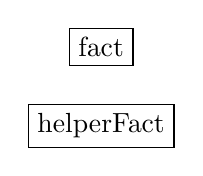
\begin{tikzpicture}[node distance = 1cm]
          \node [block]                (fact)       {\hs{fact}};
          \node [block, below of=fact] (helperFact) {\hs{helperFact}};
        \end{tikzpicture}
      };
      \node [block, right of=c2] (c3) {
        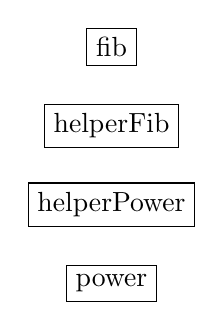
\begin{tikzpicture}[node distance = 1cm]
          \node [block]                       (fib)         {\hs{fib}};
          \node [block, below of=fib]         (helperFib)   {\hs{helperFib}};
          \node [block, below of=helperFib]   (helperPower) {\hs{helperPower}};
          \node [block, below of=helperPower] (power)       {\hs{power}};
        \end{tikzpicture}
      };
  \end{tikzpicture}
  \caption{Typical clusters for the functions in Figure \ref{fig:haskelllisp}.}
  \label{fig:haskellcluster}
\end{figure}

We have also applied our recurrent clustering algorithm to a variety of the
most-downloaded packages from \textsc{Hackage} (as of 2015-10-30), including
\texttt{text} (as above), \texttt{pandoc}, \texttt{attoparsec},
\texttt{scientific}, \texttt{yesod-core} and \texttt{blaze-html}. Whilst we
expected functions with a similar purpose to appear together, such as the
various reader and writer functions of \hs{pandoc}, there were always a few
exceptions which became separate for reasons which are still unclear.

When clustering the \hs{yesod} Web framework, the clustering did seem to match
our intuitions, in particular since all 15 of Yesod's MIME type identifiers
appeared in the same cluster.

Whilst recurrent clustering has produced results which merit further
investigation, the application to theory exploration has yet to be tested
empirically. This is due to \qspec{}'s use of \qcheck{}'s \hs{Arbitrary} type
class to generate random values for instantiating variables. Whilst we can
automatically define \qspec{} theories and invoke them with \hs{nix-eval}, not
all types have \hs{Arbitrary} instances; those without cannot be given any
variables in our signature, which severely limits the possible combinations
which can be explored. In many cases, no variables can be included at all,
leaving just equations involving constants. This has so far prevented us from
measuring the direct impact on \qspec{} performance, either directly by
exploring the sub-sets identified through recurrent clustering, or indirectly by
comparing the equations generated by a full brute-force search to our recurrent
clusters: those equations relating terms from different clusters would not be
discovered by our method. It is this ratio of equations found through brute
force to those found after narrowing-down by clusters which is one of our key
objectives to maximise at this stage; until we begin to pursue the
\emph{interestingness} of the properties.

The following less-serious problems were also encountered while applying
\textsc{ML4HS} to \textsc{Hackage} packages:

\begin{itemize}
\item Some packages, such as \texttt{warp} and \texttt{conduits}, get no
  declarations to cluster. This is because they make all of their declarations
  privately, e.g. in ``internal'' modules, then use separate modules to export
  the public declarations. GHC's renaming phase makes all references to such
  exports canonical, by pointing them to the private declarations. This forces
  us to ignore such declarations, as \qspec{} will not be able to access them.

\item Since we do not support type-level entities, we ignore type
  classes. Unfortunately, this also means ignoring any value-level bindings (AKA
  ``methods'') which occur in a type class instance. Instead of being clustered,
  these result in references getting $f_{recursion}$ features. This is
  especially noticable in libraries like \hs{scientific}, where only the
  functions for constructing and destructing numbers in scientific notation are
  clustered; all of the arithmetic is defined in type classes. One difficulty
  with supporting methods is that their namespace in Core is disjoint from that
  of regular Haskell identifiers: a transformation layer would be required,
  along with explicit type annotations to avoid ambiguity.
\end{itemize}

It seems like this recurrent clustering method has promise, although it will
require a more thorough exploration of the parameters to obtain more intuitively
reliable results. These clusters can then be used in several ways to perform
theory exploration; the most na\"{\i}ve way being to explore each cluster as
\qspec{} signature in its own right. \textsc{ML4HS} already provides this
functionality, although the lack of test generators severely limits what can be
discovered.

As alluded to previously, we also have the opportunity to reason by
\emph{analogy}. Similar to the work on ACL2(ml) \cite{heras2013proof}, we could
produce a general ``scheme'' from each equation we find (either through \qspec{}
or by data mining test suites); like Isabelle approaches have shown
\cite{Montano-Rivas.McCasland.Dixon.ea:2012}, these schemes could then be
instantiated to a variety of similar values, in an attempt to find new theorems
which are analogues of existing results from a different context. ``Mutating''
existing theorem statements in such a way would also increase the chance of any
result being considered interesting; since it's likely that the unmodified
statement was deemed interesting, and the new result would not in general follow
as a simple logical consequence.

\fi

\section{Related Work}
\label{sec:related}

\subsection{Theory Exploration}

We briefly described theory exploration in \S \ref{sec:theoryexploration}, as
the task of discovering \emph{new} theorems in a software or proof library,
rather than proving/disproving user-provided statements. This general idea dates
back at least to the 1970s, most famously to work by Lenat
\cite{lenat1977automated}, though the theory exploration tools used in
functional programming trace their roots back to the interactive
\textsc{Theorema} \cite{buchberger2000theory} system of Buchberger.

As well as \qspec{} and \hspec{} in Haskell, automated theory exploration has
been applied to Isabelle \cite{Montano-Rivas.McCasland.Dixon.ea:2012}
\cite{johansson2009isacosy} \cite{Hipster}. Since \qspec{} is used for
conjecture generation in many of these systems, they may also benefit from our
machine learning approach.

\subsection{Relevance Filtering}
\label{sec:relevance}

The idea of \emph{relevance filtering} (or, \emph{premise selection}) is to
reduce the search space of a theorem proving task by removing redundant or
irrelevant information (axioms, definitions, lemmas, etc.) from the input. Our
restriction of theory exploration to intelligently-selected clusters of symbols,
rather than whole libraries at a time, is essentially the same idea applied in a
novel setting.

The technique is used in Isabelle's Sledgehammer tool, during its translation of
Isabelle/HOL theories to statements in first order logic: rather than
translating the entire theory, only a sub-set of relevant clauses are
included. This reduces the size of the problem and speeds up the proof search,
but it creates the new problem of determining when a clause is relevant: how do
we know what will be required, before we have the proof?

The original approach uses the proportion of symbols which a clause has in
common with the problem statement \cite{meng2009lightweight} (plus various
heuristics), although various alternatives have been proposed in the literature
\cite{kuhlwein2013mash} \cite{kuhlwein2012overview} \cite{alama2014premise}.

\subsection{Recurrent Clustering}
\label{sec:clusteringexpressions}

Our recurrent clustering algorithm is similar to that of ML4PG, as our
transformation maps the elements of a syntax tree to distinct cells in a
matrix. In contrast, the matrices produced by ACL2(ml) \emph{summarise} the tree
elements: providing, for each level of the tree, the number of variables,
nullary symbols, unary symbols, etc.

Unlike ML4PG, our algorithm can handle mutually-recursive definitions, but it
also ignores types. This is because obtaining the type of each component of a
Core definition is more difficult than in ML4PG (which queries the current
\textsc{Proof General} state), and is left for future work.

The way we \emph{use} our clusters to inform theory exploration is actually more
similar to that of ACL2(ml) than ML4PG. ML4PG can either present clusters to the
user for inspection, or produce automata for recreating proofs. In ACL2(ml), the
clusters are used to restrict the search space of a proof search, much like we
restrict the scope of theory exploration.

\subsection{Feature Extraction}

One major difficulty when applying statistical machine learning algorithms to
\emph{languages}, such as Haskell, is the appearance of recursive
structures. This can lead to nested expressions of arbitrary depth, which are
difficult to compare in numerical ways. One common approach to this problem is
to represent such structures as \emph{sequences}. \emph{Recurrent neural
  networks} (RNNs) are a popular choice for processing sequences, especially
when combined with mechanisms such as \emph{long short-term memory} (LSTM) for
preserving information across long sequences \cite{hochreiter1997long}. Such
systems have been used, for example, to parse and execute computer programs
\cite{zaremba2014learning}. However, learning to parse sequences seems
inefficient considering that we already have correctly-parsed ASTs.

Whilst neural networks have been applied directly to recursive structures
\cite{goller1996learning}, including using LSTM \cite{zhu2015long}, a more
popular approach is to use \emph{kernel methods}
\cite{bakir2007predicting}. These are promising as a more principled alternative
to our current hand-crafted translation of ASTs to vectors.

\section{Conclusion and Future Work}
\label{sec:conclusion}

Our use of clustering to pre-process \qspec{} signatures has required many
decisions and tradeoffs to be made. Hence our approach is just one possibility
out of many alternatives which could be investigated to push this work further.

The most obvious next step is to incorporate types. Types contain valuable
information about an expression, and would allow us to distinguish between
constructors. Since our algorithm closely follows that of ML4PG, which
\emph{does} support types, the only barrier is the practical issue of
propagating annotations through all of the Core definitions.

More speculative directions include the use of \emph{learned} representations,
rather than our hand-crafted features \cite{bengio2013representation}. This
would provide an interesting comparison, as well as being more robust in the
face of language evolution. Another intriguing possibility is to extend the
recurrent nature of our algorithm to make use of the discovered properties
during clustering; for example, by treating the discovered equations as rewrite
rules to reduce the ASTs prior to feature extraction.

\appendix

\section{Core Syntax}\label{sec:core}

The GHC Core language is based on \fc{}, and described in detail in
\cite[Appendix C]{sulzmann2007system}. For our machine learning purposes we are
mostly interested in the syntax of reducible expressions (representing Haskell
of the form \hs{f a b \dots = \dots}), and use the simplified syntax given below
in BNF style ($[]$ and $(,)$ denote repetition and grouping, respectively):

\begin{equation}\label{eq:coresyntax}
  \begin{split}
    expr\    \rightarrow\ & \CVar\ id                          \\
                       |\ & \CLit\ literal                     \\
                       |\ & \CApp\ expr\ expr                  \\
                       |\ & \CLam\ \mathcal{L}\ expr           \\
                       |\ & \CLet\ bind\ expr                  \\
                       |\ & \CCase\ expr\ \mathcal{L}\ [alt]   \\
                       |\ & \CType                             \\
    id\      \rightarrow\ & \CLocal\       \mathcal{L}         \\
                       |\ & \CGlobal\      \mathcal{G}         \\
                       |\ & \CConstructor\ \mathcal{D}         \\
    literal\ \rightarrow\ & \CLitNum\ \mathcal{N}              \\
                       |\ & \CLitStr\ \mathcal{S}              \\
    alt\     \rightarrow\ & \CAlt\ altcon\ expr\ [\mathcal{L}] \\
    altcon\  \rightarrow\ & \CDataAlt\ \mathcal{D}             \\
                       |\ & \CLitAlt\ literal                  \\
                       |\ & \CDefault                          \\
    bind\    \rightarrow\ & \CNonRec\ binder                   \\
                       |\ & \CRec\ [binder]                    \\
    binder   \rightarrow\ & \CBind\ \mathcal{L}\ expr
  \end{split}
\end{equation}
Where:
\begin{tabular}[t]{l @{ $=$ } l}
  $\mathcal{S}$ & string literals    \\
  $\mathcal{N}$ & numeric literals   \\
  $\mathcal{L}$ & local identifiers  \\
  $\mathcal{G}$ & global identifiers \\
  $\mathcal{D}$ & constructor identifiers
\end{tabular}

The full Core language emitted by GHC (as of version 7.10.2, the latest at the
time of writing) is translated automatically to this simplified form prior to
recurrent clustering. Our major restriction is to ignore type-level entities
(such as datatype definitions, explicit casts, and differences between
types/kinds/coercions). Our implementation also handles several other forms of
literal (machine words of various sizes, individual characters, etc.), but we
omit them here for brevity as their treatment is similar to those of strings and
numerals.

\section{Rose Trees}\label{sec:rosetree}

The $toTree$ function shown below transforms Core expressions, described in
Appendix \ref{sec:core} to rose trees. We follow the presentation in
\cite{blundell2012bayesian} and define rose trees recursively as follows: $T$ is
a rose tree if $T = (f, T_1, \dots, T_{n_T})$, where $f \in \mathbb{R}$ and
$T_i$ are rose trees. $T_i$ are the \emph{sub-trees} of $T$ and $f$ is the
\emph{feature at} $T$. $n_T$ may differ for each (sub-) tree; trees where
$n_T = 0$ are \emph{leaves}.

The recursive definition is mostly routine; each repeated element (shown as
$\dots$) has an example to indicate their handling, e.g. for $\CRec$ we apply
$toTree$ to each $e_i$. We ignore values of $\mathcal{D}$, since constructors
have no internal structure for us to compare; they can only be compared based on
their types, which we do not currently support. We also ignore values from
$\mathcal{S}$ and $\mathcal{N}$ as it simplifies our later definition of $\phi$,
and we conjecture that the effect of such ``magic values'' on clustering real
code is low.

%\begin{figure}
  \begin{align*}\label{fig:totree}
    toTree(e) &=
    \begin{cases}
      (\feature{\CVar},     toTree(e_1))                                 & \text{if $e = \CVar\ e_1$} \\
      (\feature{\CLit},     toTree(e_1))                                 & \text{if $e = \CLit\ e_1$} \\
      (\feature{\CApp},     toTree(e_1), toTree(e_2))                    & \text{if $e = \CApp\ e_1\ e_2$} \\
      (\feature{\CLam},     toTree(e_1))                                 & \text{if $e = \CLam\ l_1\ e_1$} \\
      (\feature{\CLet},     toTree(e_1), toTree(e_2))                    & \text{if $e = \CLet\ e_1\ e_2$} \\
      (\feature{\CCase},    toTree(e_1), toTree(a_1), \dots)             & \text{if $e = \CCase\ e_1\ l_1\ a_1\ \dots$} \\
      (\feature{\CType})                                                & \text{if $e = \CType$} \\
      (\feature{\CLocal},   (\feature{l_1}))                            & \text{if $e = \CLocal\ l_1$} \\
      (\feature{\CGlobal},  (\feature{g_1}))                            & \text{if $e = \CGlobal\ g_1$} \\
      (\feature{\CConstructor})                                         & \text{if $e = \CConstructor\ d_1$} \\
      (\feature{\CLitNum})                                              & \text{if $e = \CLitNum\ n_1$} \\
      (\feature{\CLitStr})                                              & \text{if $e = \CLitStr\ s_1$} \\
      (\feature{\CAlt},     toTree(e_1), toTree(e_2))                   & \text{if $e = \CAlt\ e_1\ e_2\ l_1\ \dots$}  \\
      (\feature{\CDataAlt})                                             & \text{if $e = \CDataAlt\ g_1$}  \\
      (\feature{\CLitAlt},  toTree(e_1))                                & \text{if $e = \CLitAlt\ e_1$}  \\
      (\feature{\CDefault})                                             & \text{if $e = \CDefault$}  \\
      (\feature{\CNonRec},  toTree(e_1))                                & \text{if $e = \CNonRec\ e_1$}  \\
      (\feature{\CRec},     toTree(e_1), \dots)                         & \text{if $e = \CRec\ e_1\ \dots$} \\
      (\feature{\CBind},    toTree(e_1))                                & \text{if $e = \CBind\ l_1\ e_1$}
    \end{cases}
  \end{align*}

%\end{figure}
